\documentclass[12pt]{kiarticle} 
\graphicspath{{pictures/}}
\DeclareGraphicsExtensions{.pdf,.png,.jpg,.eps}
%%%
\pagestyle{fancy}
\fancyhf{}
%\renewcommand{\headrulewidth}{ 0.1mm }
\renewcommand{\footrulewidth}{ .0em }
\fancyfoot[C]{\texttt{\textemdash~\thepage~\textemdash}}
\fancyhead[L]{Некоторые концепции теоретической физики, ДЗ № 1\hfil}
\fancyhead[R]{\hfil Иванов Кирилл, 625 группа }

\newcommand{\Ll}{\ensuremath{\mathcal{L}}}


\begin{document}

\begin{titlepage}		
	\begin{center}
		\large 	Московский физико-технический институт \\
		Факультет общей и прикладной физики \\
		\vspace{0.2cm}
		Образовательная программа\\
		"<Квантовая теория поля, теория струн и математическая физика">
		
		\vspace{4.5cm}
		III семестр 2017-2018 учебного года \\ \vspace{0.1cm}
		\large Домашнее задание №1: \\ \vspace{0.1cm}
		\LARGE \textbf{Элементы классической теории поля, Лагранжев формализм}
	\end{center}
	\vspace{2.3cm} \large
	
	\begin{center}
		Автор: \\
		Иванов Кирилл,
		625 группа
		\vspace{10mm}
		
		
	\end{center}
	
	\begin{center} \vspace{50mm}
		г. Долгопрудный \\ 
		15 сентября 2017 года
	\end{center}
\end{titlepage}

%______________________________________________________________________________________________


%
%
%%%%%%%%%%%%%%%%%%%%%%%%%%%%%%%%%%%%%%%%
%
%

\section{Вопросы}


\textbf{Лагранжиан}, или функция Лагранжа --- величина, характеризующая систему,  является функцией обобщённых координат $ q_i(t) $, их производных $ \dot{q_i}(t) $ и самого времени $ t $:

\begin{equation}\label{}
\Ll = \Ll \left( q_i(t), \dot{q_i}(t), t\right) , \qquad i = 1, 2, \ldots N
\end{equation}

В механике ее физическим смыслом является разность кинетической и потенциальной энергии системы: 

\begin{equation}\label{L}
\Ll = T - U = \dfrac{m\dot{q_i}^2}{2} - U
\end{equation}

\textbf{Уравнения Лагранжа} являются аналогом 2 закона Ньютона и получаются простым дифференцированием \eqref{L} и подстановкой в 2 ЗН:

\[ 
\pdd{\Ll}{\dot{q_i}} = m\dot{q_i}, \qquad \pdd{\Ll}{q_i} = - \pdd{U}{q_i} \te
 \]
 \begin{equation}\label{E-L}
 \dfrac{d}{dt} \pdd{\Ll}{\dot{q_i}} - \pdd{\Ll}{q_i} = 0 \; \ekv \; m\ddot{q_i} = - \pdd{U}{q_i}
 \end{equation}

По определению \textbf{действием} называют интеграл вида 

\begin{equation}\label{S}
S = \int\limits_{t_1}^{t_2} \Ll(q, \dot{q}, t) dt
\end{equation}

Действие --- это функционал, физический смысл которого можно трактовать как "<количество движения">. 

Введем некую функцию $ I = I (q(t), \dot{q}(t) $, и будем называть ее \textbf{интегралом движения}, если 

\begin{equation}\label{I}
\dfrac{d I (q(t), \dot{q}(t) )}{dt} = 0 \te I (q(t), \dot{q}(t) ) = \co 
\end{equation}


%%%
%%%%%
%%%%%%%%
%%%%%%

\section{Упражнения}

\subsection{Упражнение 1}

\textbf{Принцип наименьшего действия} заключается в том, что если у нас есть определённые положения системы $ q(t_1) $ и $ q(t_2) $, то между двумя этими положениями система движется так, чтобы интеграл \eqref{S} имел минимальное (или экстремальное в более общем случае) значение. 

Произведём вариации, т.е. добавим к координате бесконечно малый член $ \delta $, т.е. $ q(t) \st q(t) + \delta q(t) $. При этом наложим граничное условие 

\begin{equation}\label{dq}
\delta q(t_1) = \delta q (t_2) = 0
\end{equation}

Тогда математически принцип наименьшего действия формулируется как

\begin{equation}\label{dS}
\delta S = S(q + \delta q, \dot{q} + \delta \dot{q}) - S (q, \dot{q}) = 0
\end{equation}

Подставим в \eqref{dS} определение действия \eqref{S}: 

\begin{equation}\label{}
 \delta S= \int\limits_{t_1}^{t_2} \left[ \Ll(q + \delta q, \dot{q} + \delta \dot{q})  -  \Ll(q, \dot{q}) \right]  dt = \int\limits_{t_1}^{t_2} \left [ \pdd{\Ll}{q}\delta q + \pdd{\Ll}{\dot{q}}\delta\dot{q} \right ] dt =  \int\limits_{t_1}^{t_2} \left [ \pdd{\Ll}{q}\delta q + \pdd{\Ll}{\dot{q}} \dfrac{d}{dt}\delta q \right ] dt
\end{equation}

Теперь проинтегрируем по частям и воспользуемся условием \eqref{dq}:

\begin{equation}\label{}
\delta S = \int\limits_{t_1}^{t_2} \left [ \pdd{\Ll}{q}\delta q - \dfrac{d}{dt} \pdd{\Ll}{\dot{q}} \delta q \right ] dt + \pdd{\Ll}{\dot{q}} \delta q \; \bigg |_{t_1}^{t_2} =  \int\limits_{t_1}^{t_2} \left [ \pdd{\Ll}{q} - \dfrac{d}{dt} \pdd{\Ll}{\dot{q}}  \right ]\delta q dt  = 0
\end{equation}

Отсюда мы и получаем исходные уравнения Лагранжа \eqref{E-L}. 


\subsection{Упражнение 2}

Пусть у нас координата $ q(t) $ варьируется как $ q(t) \st q(t) + \epsilon h(t) $, где $ \epsilon \ll 1 $. Тогда существование 

\begin{equation}\label{Sym}
\delta \Ll = \Ll (q(t) + \epsilon h(t)) - \Ll (q(t)) = 0 
\end{equation}

называется симметрией системы. \textbf{Теорема Нетер} утверждает, что если существует симметрия \eqref{Sym}, то будет существовать и интеграл движения \eqref{I}. 

\paragraph{Док-во.} Предположим, что наше действие из \eqref{dS} зависит от некой функции, подобной лагранжиану, умноженной на некую добавку $ \dot{\epsilon} $, зависящую в общем случае от времени:

\begin{equation}\label{}
\delta S = 0 = \int\limits_{t_1}^{t_2} I(q, \dot{q}) \dot{\epsilon} dt =  \int\limits_{t_1}^{t_2} I(q, \dot{q}) d\epsilon = I(q, \dot{q})\epsilon \; \bigg |_{t_1}^{t_2} -   \int\limits_{t_1}^{t_2} I(q, \dot{q}) dt = 0
\end{equation}

Из физического смысла понятно, что согласно определениям из \eqref{dq} и \eqref{Sym} это равносильная запись принципа наименьшего действия \eqref{dS}. Пользуясь для $ \epsilon $ условием (5), мы обнуляем первый член и получаем требуемое доказательство:

\begin{equation}\label{}
\int\limits_{t_1}^{t_2} I(q, \dot{q}) dt = 0 \qquad \te \dfrac{dI(q, \dot{q})}{dt} = 0 \te I(q, \dot{q} ) = 0
\end{equation}





\section{Задачи}

\subsection{Задача 1}

\begin{wrapfigure}{l}{0.34\linewidth} 
	
	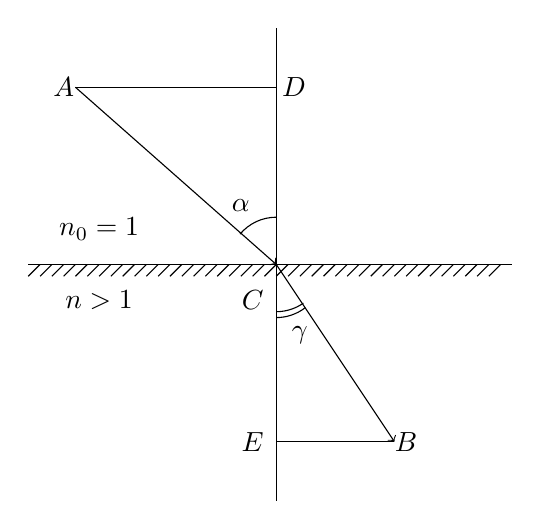
\begin{tikzpicture} [scale = 1.5,]
	 \draw  (-2.1, 0) -- (2, 0);
	 \draw [->] (-1.7, 1.5) -- (0, 0);
	 \draw (-1.7, 1.5) -- (0, 1.5);
	 \draw  [<-] (1, -1.5) -- (0, 0);
	  \draw   (1, -1.5) -- (0, -1.5);
	 \draw (0, 2) -- (0, -2);
	  \draw (0, 0.4) arc (90:140: 0.4);
	   \draw (0, -0.4) arc (270:305: 0.4);
	      \draw (0, -0.45) arc (270:308: 0.4);
%	\draw (-2.1, 0) -- (2, 0);
	\foreach \x in {-2, -1.9, ..., 2} \draw (\x, 0) -- + (-0.1, -0.1); 
	\draw (-1.8,1.5) node {$ A$};
		\draw (0.15,1.5) node {$ D$};
			\draw (-0.2,-1.5) node {$ E$};
	\draw (1.1,-1.5) node {$ B $};
		\draw (-0.2,-0.3) node {$ C$};
	\draw (-0.3,0.5) node {$ \alpha $};
	\draw (-1.5,0.3) node {$ n_0 = 1 $};
		\draw (-1.5,-0.3) node {$ n > 1 $};
		\draw (0.2,-0.6) node {$ \gamma $};
%	\draw (-0.7, 0)  rectangle + (1.4, 0.8); 
%	\draw [->] (0.7, 0.35) -- (1.7, 0.35) node[anchor=west] {$ \vec{F} $};
%	\draw (0, 0.4)  node {$ m $};
	
	\end{tikzpicture}
	\caption{Преломление света}
\end{wrapfigure}

Выведем закон преломления света, опираясь на предположение, что луч света бежит по пути, занимающему наименьшее время.. Нам известно, что свет идет из среды с показателем преломления $ n_0 =1  $ в среду с показателем $ n > 1 $. Он проходит через точку $ C $ так, чтобы его путь занимал наименьшее время. 

Он проходит путь $ AC + CB $ за время $ \tau = \dfrac{AC}{c} + \dfrac{BC}{v} \hm{=} \dfrac{AC + nCB}{c} $. Пусть мы знаем $ AD + EB = L, DC, CE $. Будем считать $ EB = x $ -- переменной, и тогда очевидно, что $ AD = L - x $. Из теоремы Пифагора получаем 

\begin{equation}\label{}
\tau = \dfrac{1}{c} \left( \sqrt{DC^2 + (L - x)^2} + n\sqrt{CE^2 + x^2} \right) 
\end{equation}

Возьмем производную по времени от переменной $ x $ и приравняем ее к нулю для нахождения экстремума:

\begin{equation}\label{}
\dfrac{d\tau}{dx} = \dfrac{1}{c} \left( n\dfrac{x}{\sqrt{CE^2 + x^2} } - \dfrac{L - x}{\sqrt{DC^2 + (L - x)^2}} \right) =0 \te n \dfrac{EB}{BC} = \dfrac{AD}{AC}
\end{equation}

Так как из геометрии $ \sin \alpha = \dfrac{AD}{AC}, \sin \gamma = \dfrac{x}{CB} $, получаем искомый закон преломления света:

\begin{equation}\label{}
\sin \alpha = n\sin \gamma
\end{equation}

\subsection{Задача 2}

В сферических координатах известно, что 

\begin{equation}\label{}
x = r\sin\theta\cos\phi, \quad
y = r\sin\theta\sin\phi, \quad
z = r\cos\theta.
\end{equation}

Здесь $ (r, \phi, \theta) \ekv (q_1, q_2, q_3)$. Легко получить и выражение для скоростей и кинетической энергии системы: $ v_r = \dot{r}, v_\phi = r\sin\theta\dot{\phi}, v_\theta = r\dot{\theta} $, тогда 

\begin{equation}\label{}
 T = \dfrac{1}{2} mv^2 = \dfrac{1}{2} m( \dot{r}^2 + r^2\sin^2\theta\dot{\phi}^2 + r^2\dot{\theta}^2)
\end{equation}

Отсюда мы получаем запись Лагранжиана:

\begin{equation}\label{}
\Ll = T - U = \dfrac{1}{2} m( \dot{r}^2 + r^2\sin^2\theta\dot{\phi}^2 + r^2\dot{\theta}^2) - \dfrac{k}{r}
\end{equation}

Тогда продифференцируем $ \pdd{\Ll}{q_i}, \pdd{\Ll}{\dot{q_i}}, \frac{d}{dt}  \pdd{\Ll}{\dot{q_i}} $ и запишем систему из трех уравнений Лагранжа:

\begin{equation}\label{}
\sys{
	& m\ddot{r} - mr\dot{\theta}^2 - mr\sin^2\theta\dot{\phi}^2 = \dfrac{k}{r^2} \\
	& 2\sin\theta\dot{\phi} + 2r\cos\theta\dot{\theta}\dot{\phi} + r\sin\theta\ddot{\phi} = 0 \\
	& r\ddot{\theta} + 2r\dot{\theta} - r\sin\theta\cos\theta\dot{\phi}^2 = 0
}
\end{equation} 

\subsection{Задача 3}

Будем решать задачу в декартовых координатах, где Лагранжиан равен

\begin{equation}\label{Lxyz}
\Ll = \dfrac{1}{2}m (\dot{x}^2 + \dot{y}^2 + \dot{z}^2 ) - \dfrac{k}{\sqrt{x^2 + y^2 +z^2}}
\end{equation}

Будем считать поворот как композицию поворотов вокруг осей $ x, y, z $. Например, повернув на угол $ \alpha $ вокруг оси $ z $, мы получаем замену координат 

\begin{equation}\label{pov_z}
\sys{
	& x' = x\cos\alpha -y\sin\alpha\\
	& y' = x\sin\alpha + y\cos\alpha\\
	& z' = z
}
\te
\sys{
	& \dot{x'} = \dot{x}\cos\alpha - \dot{y}\sin\alpha\\
	& \dot{y'} = \dot{x}\sin\alpha + \dot{y}\cos\alpha\\
	& \dot{z'} = \dot{z}
}
\end{equation}

Простой подстановкой в \eqref{Lxyz} нетрудно убедиться в инвариантности вида Лагранжиана в штрихованных координатах. Аналогично проверятся для 2 и 3 поворота вокруг осей $ x, y $. 

Бесконечно-малые преобразования получаются, если мы считаем $ \alpha \ll 1 \te \cos\alpha \hm{\approx} 1, \sin\alpha \approx \alpha $:

\begin{equation}\label{pov_z_bm}
\sys{
	& x' = x -y\alpha\\
	& y' = x\alpha + y\\
	& z' = z
}
\te
\sys{
	& \dot{x'} = \dot{x} - \dot{y}\alpha\\
	& \dot{y'} = \dot{x}\alpha + \dot{y}\\
	& \dot{z'} = \dot{z}
}
\end{equation}

Запишем теперь в матричном виде для всех трех поворотов: 

\begin{equation}\label{}
M_x(\alpha) =
\begin{pmatrix}
1 & 0 & 0  \\
0 & 1 & -\alpha  \\ 
0 & \alpha & 1  \\
\end{pmatrix}, \quad
M_y(\beta) =
\begin{pmatrix}
1 & 0 & \beta  \\
0 & 1 & 0  \\ 
-\beta & 0 & 1  \\
\end{pmatrix}, \quad
M_z(\gamma) =
\begin{pmatrix}
1 & -\gamma & 0  \\
\gamma & 1 & 0  \\ 
0 & 0 & 1  \\
 \end{pmatrix}, \quad
\end{equation}

Тогда единая матрица поворота будет произведением этих трех. Запишем ее, отбрасывая порядки малости больше первого: 

\begin{equation}\label{}
M(\alpha, \beta, \gamma) = \begin{pmatrix}
1 & -\gamma & -\beta  \\
\gamma & 1 & -\alpha  \\ 
\beta & \alpha & 1  \\
\end{pmatrix}
\te 
\begin{pmatrix}
x' \\
y' \\
z'
\end{pmatrix}
=
\begin{pmatrix}
1 & -\gamma & -\beta  \\
\gamma & 1 & -\alpha  \\ 
\beta & \alpha & 1  \\
\end{pmatrix}
\begin{pmatrix}
x \\
y \\
z
\end{pmatrix}
\end{equation}

\end{document}